\begin{figure*}%[!hbtp]
	\centering
	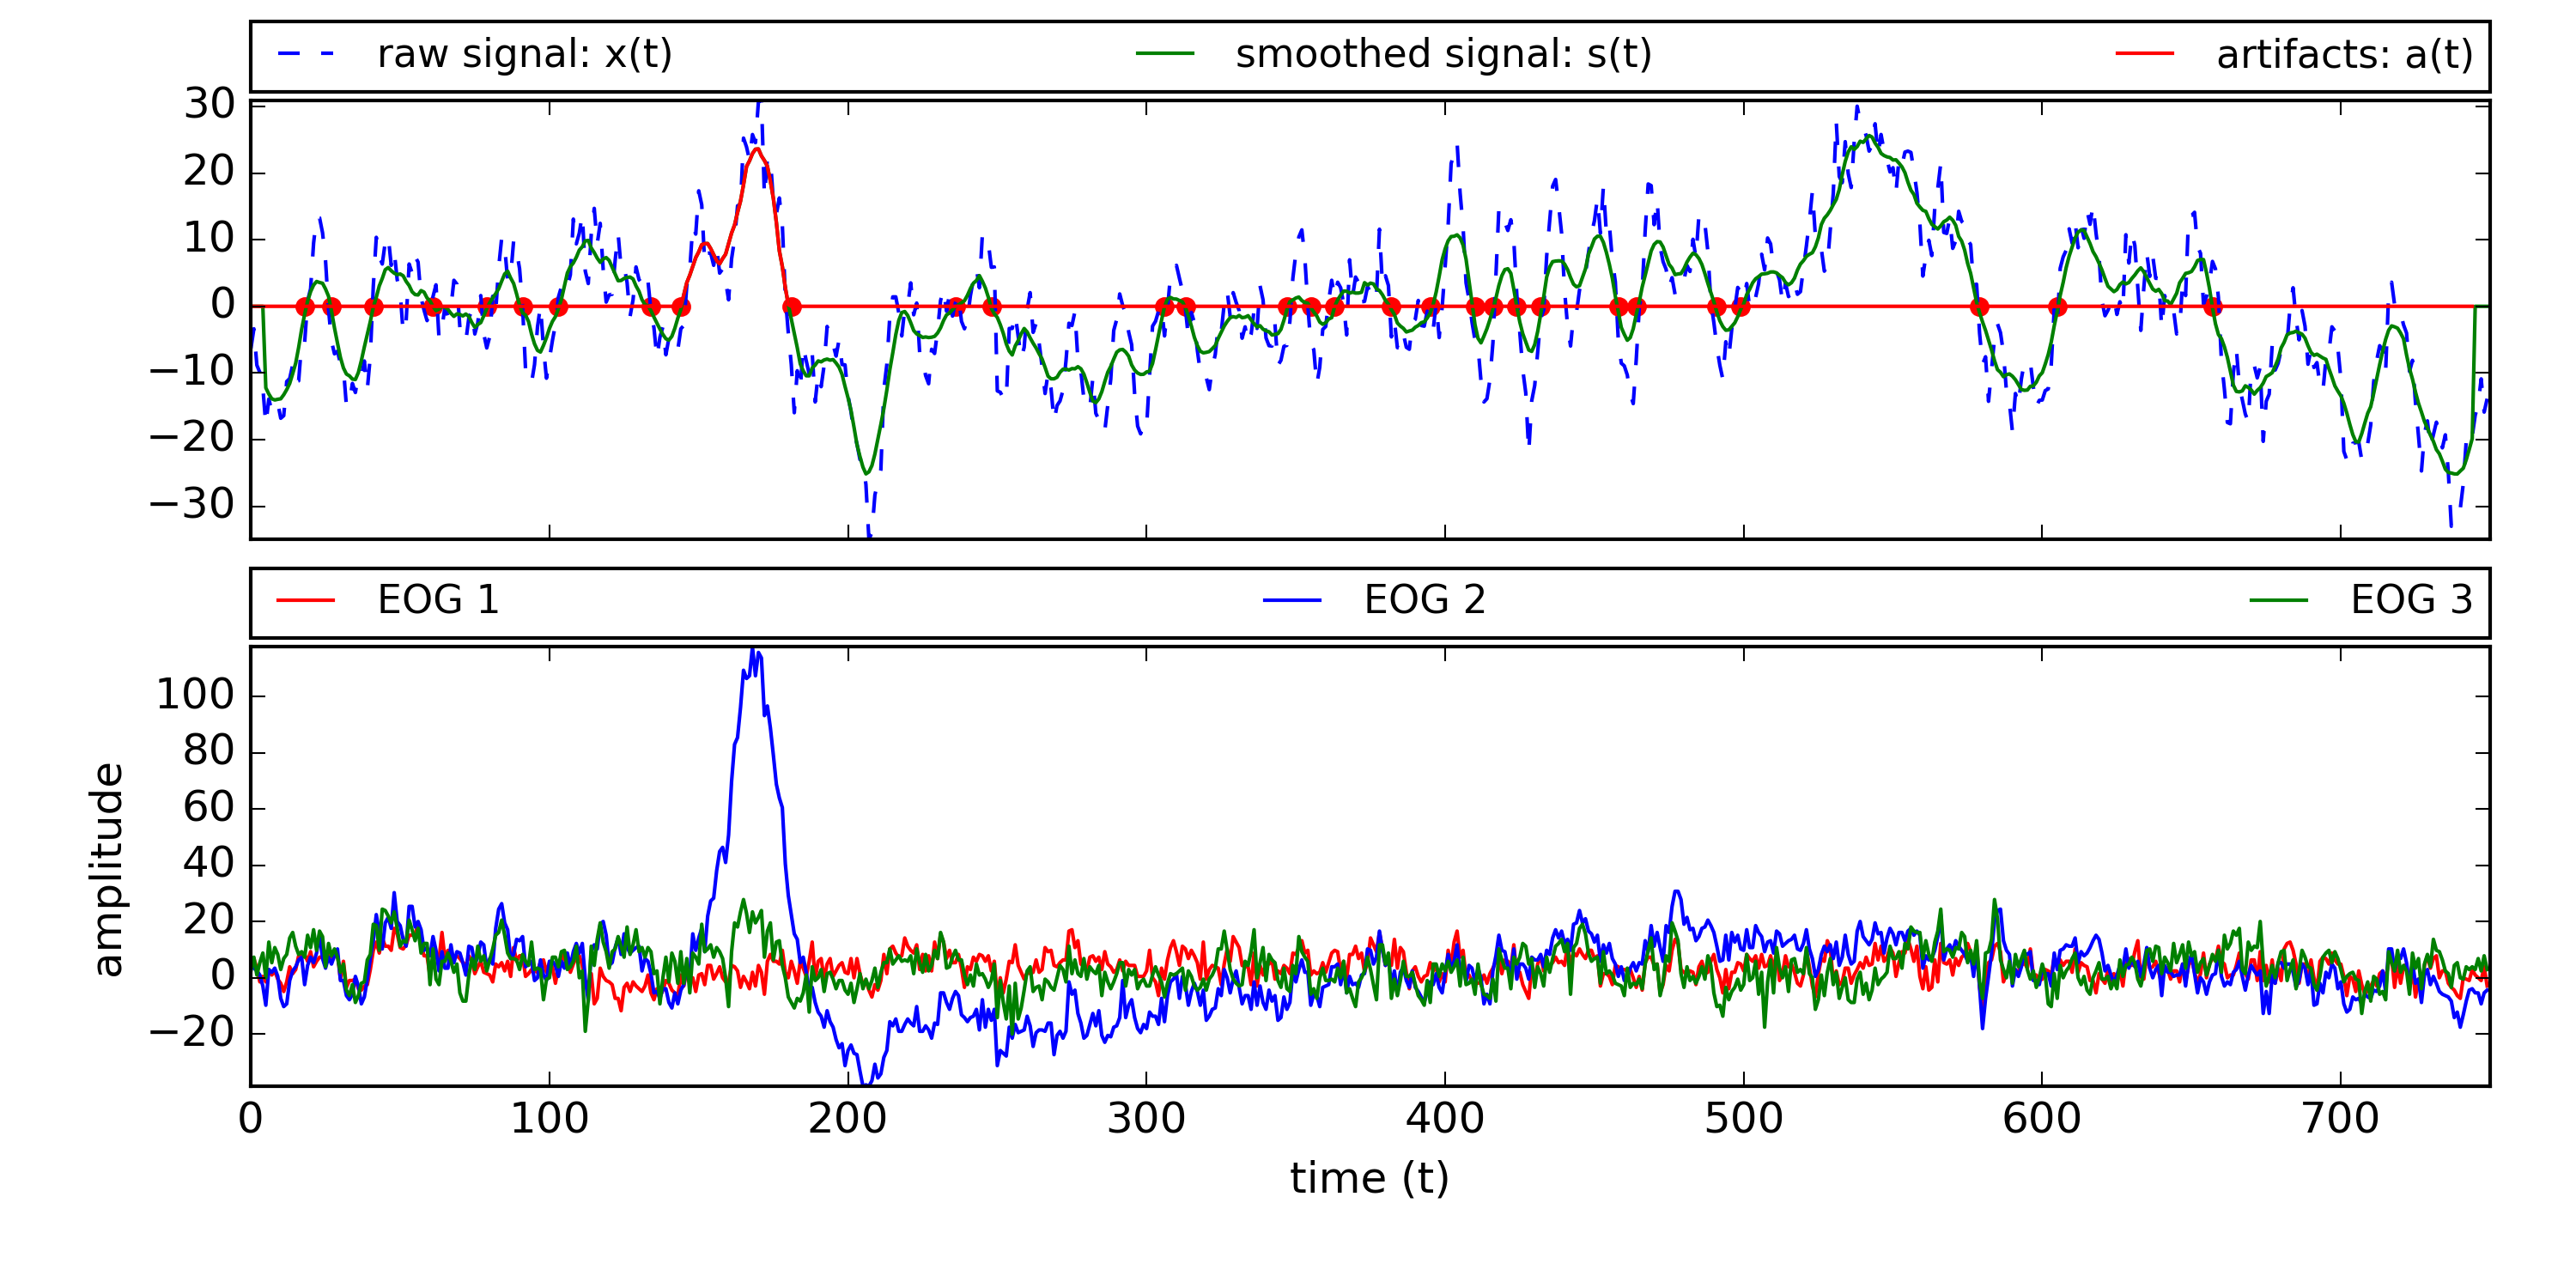
\includegraphics[width=1\textwidth]{figures/oacl-signals.png}
	\vspace{-2em}
	\caption{Top: smoothed signal and artifact signal superimposed on the raw EEG signal for a single channel in part of a single trial. The red artifact signal shows correct detection of artifact in this trial. Bottom: Three EOG signals showing ocular artifacts.}
	\label{fig:oacl-signals}
\end{figure*}
\section{Ocular Artifact Correction}\label{sec:oacl}
The ocular artifact correction method OACL consists of two parts: artifact detection and artifact removal \citep{li2015ocular}. First, the raw EEG signals are processed to obtain the artifact signals, representing the parts of the signal that are artifacts. Then we find the \emph{filtering parameter} $\theta$ for each of the artifact signals. $\theta$ determines the amount of an artifact signal that needs to be removed from the raw signal in order to correct it. Since the OACL method was originally designed for binary class datasets, we generalize the algorithm for multi-class datasets.

An EEG signal is a sequence of $n$ samples. Let $x = (s_0,...,s_t,...,s_n)$ where $s_t \in \mathbb{R}$ denotes the EEG sample for a channel. For simplicity, we can interpret $x$ as a function $x : \mathbb{N}_{\geq 0} \rightarrow \mathbb{R}$ where $x(t)$ denotes the amplitude of $x$ at time $t$. From $x(t)$ we perform all steps in artifact detection and removal.

%Let $t \in \mathbb{N}_{\geq 0}$ be the time of a EEG sample, then $x(t)$ denotes the amplitude measured at time $t$, that is, $x(t)$ denotes the raw EEG signal for some channel.

\subsection{Artifact Detection}
The goal of artifact detection is to find an artifact signal $a(t)$ from $x(t)$ that represents the parts of $x(t)$ that contain ocular artifacts. Before finding the artifact signal $a(t)$, we first obtain a smoothed signal by applying a \emph{moving average filter} to $x(t)$, in order to smooth out short-term fluctuations e.g. from external interference. A moving average filter is a function $s: \mathbb{N} \rightarrow \mathbb{R}$ that given time t, computes the average of $\frac{m}{2}$ samples on either side of the t\textsuperscript{th} sample. 

\begin{equation}
\label{eq:movavg}
s(t) = \frac{1}{m}\sum_{t-\frac{m}{2}}^{t+\frac{m}{2}}x(t)
\end{equation}
where $m$ is an odd number of points used to smooth the signal. The raw signal $x(t)$ and the corresponding smoothed signal $s(t)$ are illustrated in \cref{fig:oacl-signals}. 

From the smoothed signal $s(t)$ the OACL method finds the changes in amplitude between the samples, which could indicate eye movement. Therefore, we proceed by computing the relative heights between samples as the maximal difference in amplitude between a sample at time $t$ and its neighboring samples, as shown in \cref{eq:relheights}.

\begin{align*}
\Delta (t) = max(&|s(t)-s(t-1)|,\\
&|s(t+1) - s(t)|) \numberthis \label{eq:relheights}
\end{align*}
where we can consider $\Delta(t)$ as describing the fluctuations in the signal.

Now, we want to have some measure of what an artifact signal looks like. \citet{li2015ocular} found by inspection that ocular artifacts generally occur with sudden changes in amplitude ($\Delta$) measured in $\mu V$ in the intervals $]30; 70[$ and $]70; 150[$. The problem with this approach is, that it does not generalize to data collected using different setups for the EEG measurement. For this reason, we automatically estimate the ranges by considering them parameters to be optimized through Bayesian Optimization, discussed in \cref{sec:bayesian-optimization}.
For now, assume that we have some range $r \in R$ where
\begin{equation}\label{eq:ranges}
R=\{(l, u) \ | \ l,u \in \mathbb{N}_{\geq 0} \text{ and } l \leq u \}
\end{equation}
Note that we can have an arbitrary number of ranges; one for each artifact characteristic. For brevity, assume we have a single range r.

Now we can find the sample indexes $t$ where $\Delta (t)$  lies in the range $r$:
\begin{align*}
P = \{t \ | \ &\frac{m}{2} < t < n-\frac{m}{2}  \quad \textnormal{and} \\
& l < \Delta (t) < u\} \numberthis \label{eq:peaks}
\end{align*}
where $n$ is the number of samples in $x(t)$, and $P$ contains the indexes of samples in $s(t)$ where a change in amplitude lies within the range that characterizes an ocular artifact.

We now have the peaks of the ocular artifacts in $s(t)$, but we still need all of the artifact before we can correct it. The approach in the OACL method is to define the artifact to be from the closest zero point before the peak, to the closest zero point after the peak. We can now find the artifact signal as
\begin{equation}\label{eq:artifactsignal}
a(t) =
\begin{cases}
s(t)      & \quad \text{if } z_b \leq t < z_a\\
0  & \quad \text{otherwise}\\
\end{cases}
\end{equation}
where $z_b, z_a$ are the zero points before and after respectively. The concept of zero points of an artifact are illustrated in \cref{fig:oacl-signals}, where zero points can be seen as red dots. 

Zero points are found from the smoothed signal, by iterating through P, finding zero-crossings from sample to sample. 
Let again $s(t)$ be the function for the smoothed signal defined in \cref{eq:movavg}. We now iterate through all values of $t$, where $t \in P$, finding $Z \subset P$ as 
\begin{align*}
Z = \{t \ | \ s(t) \leq 0 \Rightarrow &(s(t+1) > 0 \ \vee \\
& s(t-1) > 0)\}
\numberthis\label{eq:zero_points}
\end{align*}
$Z$ will then be a list of indexes $\{z_1,...z_m\}$, that is used as the zero points $z_b$ and $z_a$ in \cref{eq:artifactsignal}. We can then find the correct zero points for a given peak, by finding predecessor and successor indexes in $Z$ for the index of a given peak in the artifact signal.

Recalling that we can use an arbitrary number of ranges in \cref{eq:ranges}, we obtain the set of artifact signals for a single channel of a single trial as:
\begin{equation}\label{eq:artifact-signals}
A(t)=  \begin{pmatrix}
a_1(t) \\
a_2(t) \\
\vdots  \\
a_l(t) 
\end{pmatrix}
\end{equation}
where $a_i(t)$ is the artifact signal found with the ith range and $l$ is the number of ranges.
The idea behind this, is that different types of artifacts can be found by using different ranges. 
\subsection{Artifact Removal}
With the artifact signals $A(t)$ extracted from the raw EEG data the next task is to remove the artifacts characterized by $A(t)$ from the original signal $x(t)$. Since signals are closed under subtraction we can obtain the corrected signal $c(t)$ by subtracting artifact signal from the EEG signal as
\begin{equation}\label{eq:corrected-signal}
c(t) = x(t) - \theta^T A(t)
\end{equation}
where $\theta \in \mathbb{R}^{k}$ is the \emph{filtering parameter}. $\theta$ is a vector with the factors determining the percentage of the artifact signal to subtract from the raw signal. 

The original approach of OACL is to obtain the $\theta$ parameter by training a binary logistic regression classifier with a modified hypothesis function. In this hypothesis function, the latent variable is derived from the power of the raw signal. Instead, we consider $\theta$ parameters as hyperparameters to the ocular artifact detection, which means that we can find the values for $\theta$ by optimizing them through the Bayesian optimization algorithm. In short, this means that we find the corrected signals for one subject as
\begin{align}\label{eq:corrected-signals}
C(t)=  \begin{pmatrix}
c_1(t) \\
\vdots  \\
c_{k}(t) 
\end{pmatrix}
\end{align}
where $k$ is the number of channels. By \cref{eq:corrected-signals} this means that the number of $\theta$ parameters we optimize over is $k \times l$, where $l$ is the number of artifact signals in \cref{eq:artifact-signals}. As we expect to remove 0-100\% of the artifact signal from the raw signal, we constrain $\theta \in \mathbb{R}^{l\times n}_{[0,1]}$.

With the EEG signal corrected for artifacts, we can proceed to extract the features for classification.
\begin{figure*}%[!hbtp]
	\centering
	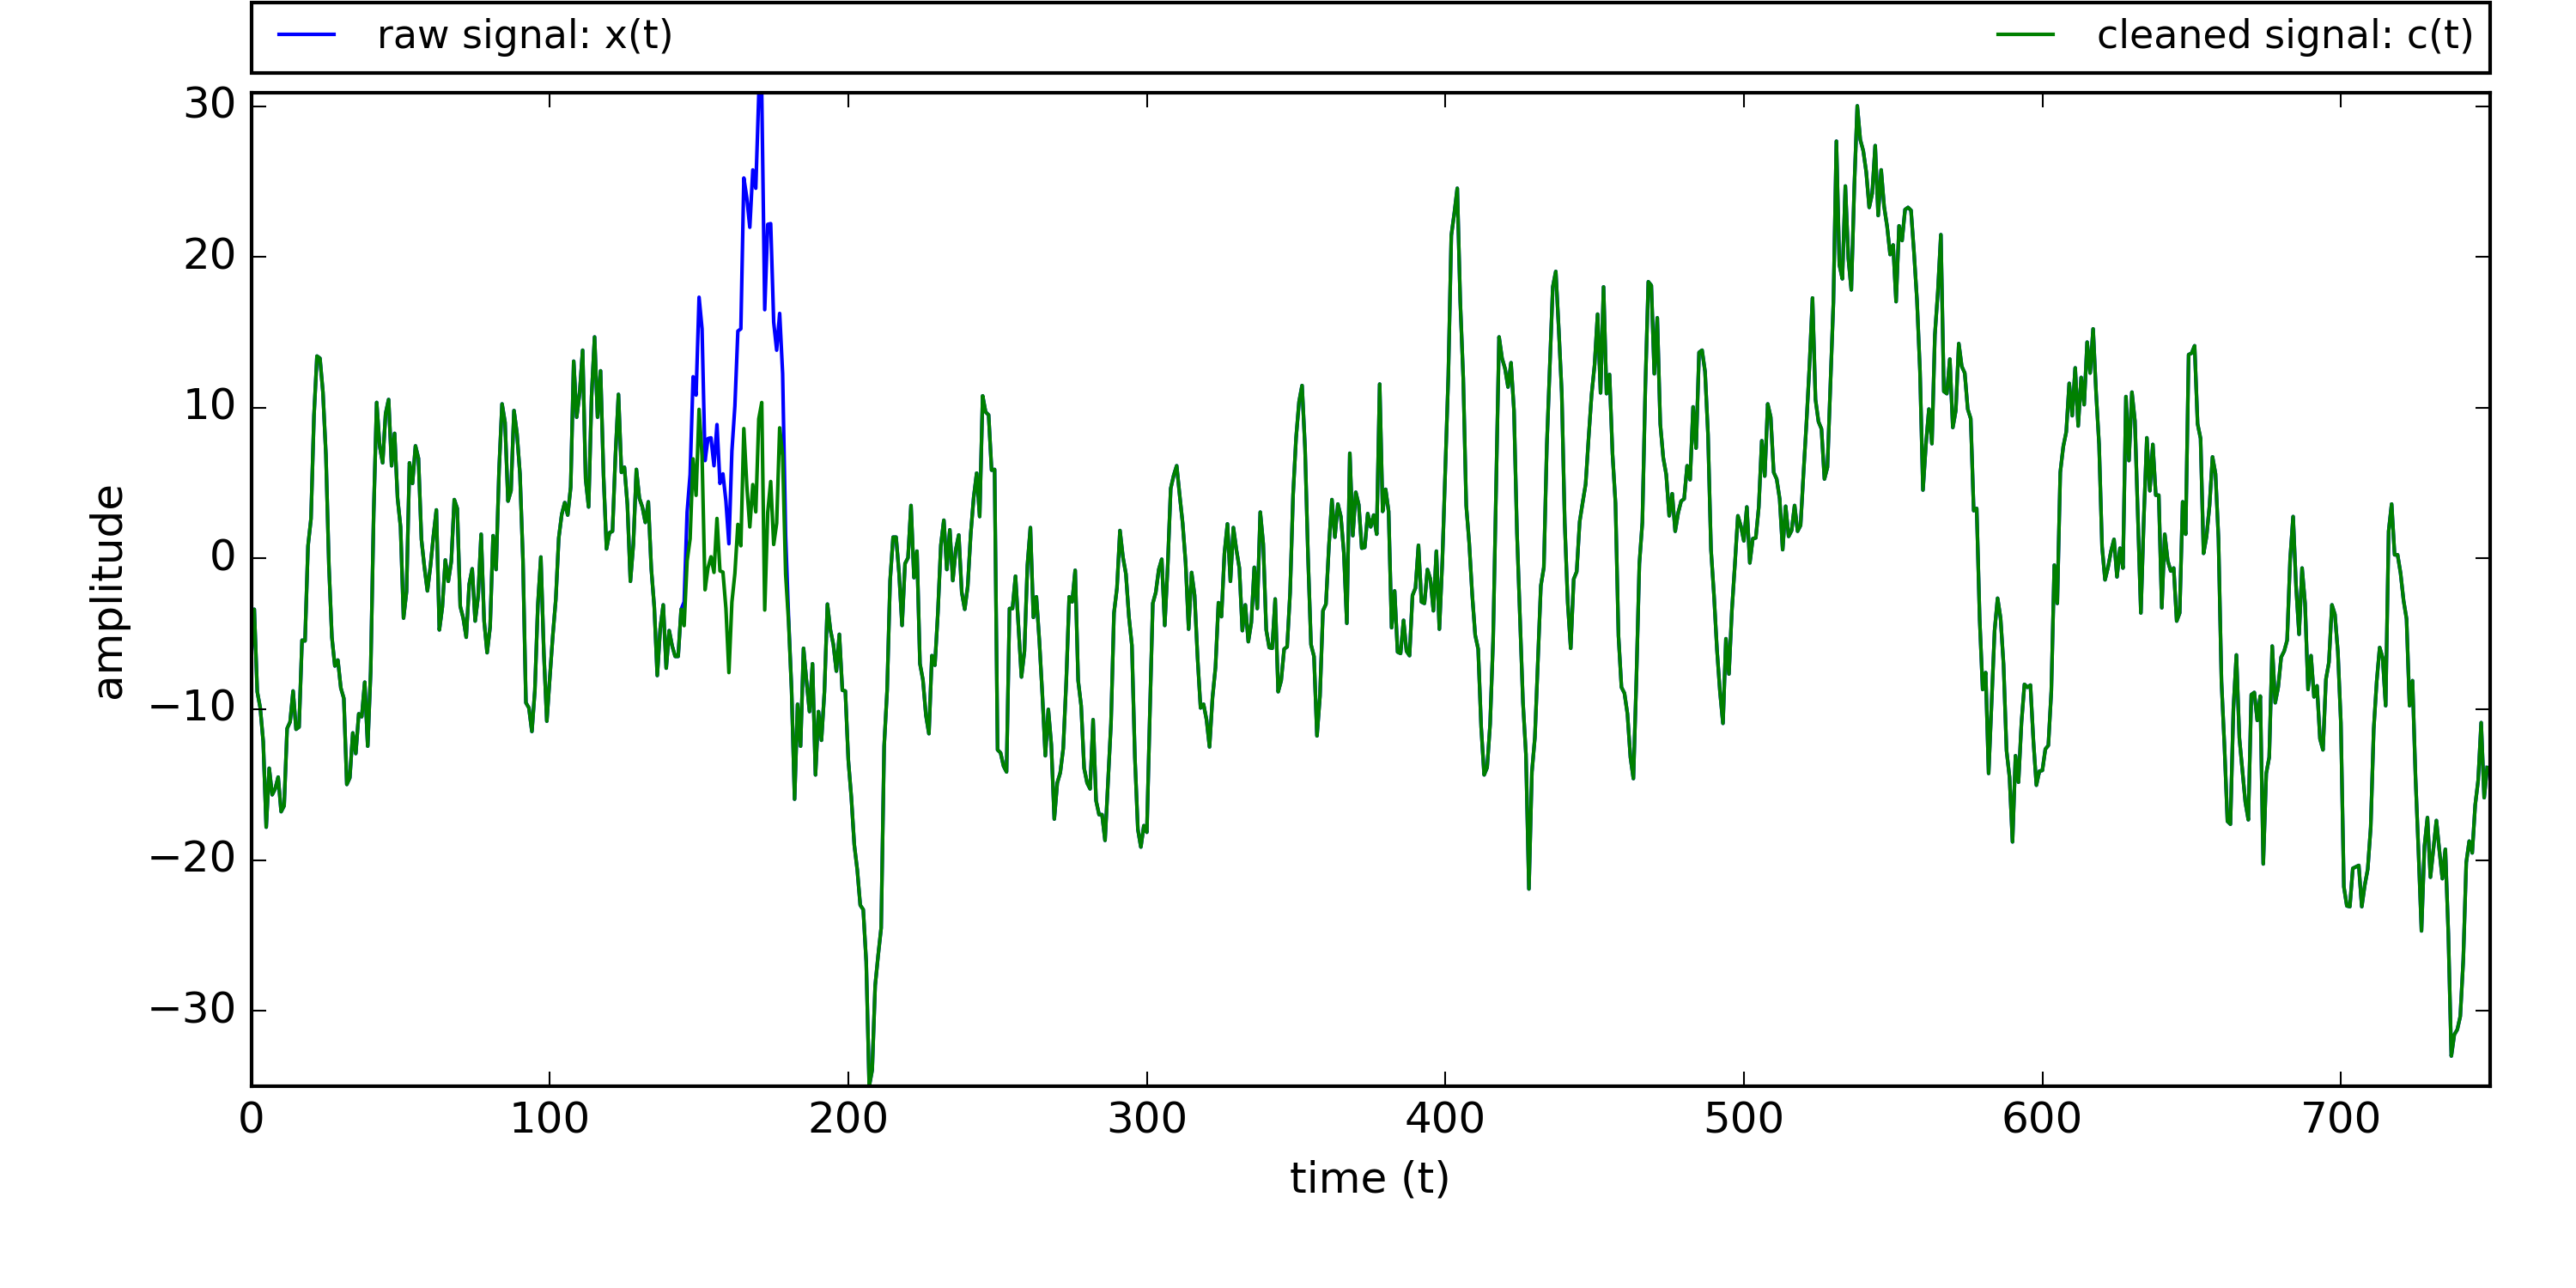
\includegraphics[width=1\textwidth]{figures/cleaned-oacl-signal.png}
	\vspace{-2em}
	\caption{Raw signal from \cref{fig:oacl-signals} and corrected signal superimposed.}
	\label{fig:cleaned-oacl-signals}
\end{figure*}